\documentclass[]{article}
\usepackage{lmodern}
\usepackage{amssymb,amsmath}
\usepackage{ifxetex,ifluatex}
\usepackage{fixltx2e} % provides \textsubscript
\ifnum 0\ifxetex 1\fi\ifluatex 1\fi=0 % if pdftex
  \usepackage[T1]{fontenc}
  \usepackage[utf8]{inputenc}
\else % if luatex or xelatex
  \ifxetex
    \usepackage{mathspec}
  \else
    \usepackage{fontspec}
  \fi
  \defaultfontfeatures{Ligatures=TeX,Scale=MatchLowercase}
\fi
% use upquote if available, for straight quotes in verbatim environments
\IfFileExists{upquote.sty}{\usepackage{upquote}}{}
% use microtype if available
\IfFileExists{microtype.sty}{%
\usepackage{microtype}
\UseMicrotypeSet[protrusion]{basicmath} % disable protrusion for tt fonts
}{}
\usepackage[margin=1in]{geometry}
\usepackage{hyperref}
\hypersetup{unicode=true,
            pdftitle={Class06 Homework Assignment: Writing a function to analyze protein-drug interactions},
            pdfauthor={Madeline R. Luth},
            pdfborder={0 0 0},
            breaklinks=true}
\urlstyle{same}  % don't use monospace font for urls
\usepackage{color}
\usepackage{fancyvrb}
\newcommand{\VerbBar}{|}
\newcommand{\VERB}{\Verb[commandchars=\\\{\}]}
\DefineVerbatimEnvironment{Highlighting}{Verbatim}{commandchars=\\\{\}}
% Add ',fontsize=\small' for more characters per line
\usepackage{framed}
\definecolor{shadecolor}{RGB}{248,248,248}
\newenvironment{Shaded}{\begin{snugshade}}{\end{snugshade}}
\newcommand{\KeywordTok}[1]{\textcolor[rgb]{0.13,0.29,0.53}{\textbf{{#1}}}}
\newcommand{\DataTypeTok}[1]{\textcolor[rgb]{0.13,0.29,0.53}{{#1}}}
\newcommand{\DecValTok}[1]{\textcolor[rgb]{0.00,0.00,0.81}{{#1}}}
\newcommand{\BaseNTok}[1]{\textcolor[rgb]{0.00,0.00,0.81}{{#1}}}
\newcommand{\FloatTok}[1]{\textcolor[rgb]{0.00,0.00,0.81}{{#1}}}
\newcommand{\ConstantTok}[1]{\textcolor[rgb]{0.00,0.00,0.00}{{#1}}}
\newcommand{\CharTok}[1]{\textcolor[rgb]{0.31,0.60,0.02}{{#1}}}
\newcommand{\SpecialCharTok}[1]{\textcolor[rgb]{0.00,0.00,0.00}{{#1}}}
\newcommand{\StringTok}[1]{\textcolor[rgb]{0.31,0.60,0.02}{{#1}}}
\newcommand{\VerbatimStringTok}[1]{\textcolor[rgb]{0.31,0.60,0.02}{{#1}}}
\newcommand{\SpecialStringTok}[1]{\textcolor[rgb]{0.31,0.60,0.02}{{#1}}}
\newcommand{\ImportTok}[1]{{#1}}
\newcommand{\CommentTok}[1]{\textcolor[rgb]{0.56,0.35,0.01}{\textit{{#1}}}}
\newcommand{\DocumentationTok}[1]{\textcolor[rgb]{0.56,0.35,0.01}{\textbf{\textit{{#1}}}}}
\newcommand{\AnnotationTok}[1]{\textcolor[rgb]{0.56,0.35,0.01}{\textbf{\textit{{#1}}}}}
\newcommand{\CommentVarTok}[1]{\textcolor[rgb]{0.56,0.35,0.01}{\textbf{\textit{{#1}}}}}
\newcommand{\OtherTok}[1]{\textcolor[rgb]{0.56,0.35,0.01}{{#1}}}
\newcommand{\FunctionTok}[1]{\textcolor[rgb]{0.00,0.00,0.00}{{#1}}}
\newcommand{\VariableTok}[1]{\textcolor[rgb]{0.00,0.00,0.00}{{#1}}}
\newcommand{\ControlFlowTok}[1]{\textcolor[rgb]{0.13,0.29,0.53}{\textbf{{#1}}}}
\newcommand{\OperatorTok}[1]{\textcolor[rgb]{0.81,0.36,0.00}{\textbf{{#1}}}}
\newcommand{\BuiltInTok}[1]{{#1}}
\newcommand{\ExtensionTok}[1]{{#1}}
\newcommand{\PreprocessorTok}[1]{\textcolor[rgb]{0.56,0.35,0.01}{\textit{{#1}}}}
\newcommand{\AttributeTok}[1]{\textcolor[rgb]{0.77,0.63,0.00}{{#1}}}
\newcommand{\RegionMarkerTok}[1]{{#1}}
\newcommand{\InformationTok}[1]{\textcolor[rgb]{0.56,0.35,0.01}{\textbf{\textit{{#1}}}}}
\newcommand{\WarningTok}[1]{\textcolor[rgb]{0.56,0.35,0.01}{\textbf{\textit{{#1}}}}}
\newcommand{\AlertTok}[1]{\textcolor[rgb]{0.94,0.16,0.16}{{#1}}}
\newcommand{\ErrorTok}[1]{\textcolor[rgb]{0.64,0.00,0.00}{\textbf{{#1}}}}
\newcommand{\NormalTok}[1]{{#1}}
\usepackage{graphicx,grffile}
\makeatletter
\def\maxwidth{\ifdim\Gin@nat@width>\linewidth\linewidth\else\Gin@nat@width\fi}
\def\maxheight{\ifdim\Gin@nat@height>\textheight\textheight\else\Gin@nat@height\fi}
\makeatother
% Scale images if necessary, so that they will not overflow the page
% margins by default, and it is still possible to overwrite the defaults
% using explicit options in \includegraphics[width, height, ...]{}
\setkeys{Gin}{width=\maxwidth,height=\maxheight,keepaspectratio}
\IfFileExists{parskip.sty}{%
\usepackage{parskip}
}{% else
\setlength{\parindent}{0pt}
\setlength{\parskip}{6pt plus 2pt minus 1pt}
}
\setlength{\emergencystretch}{3em}  % prevent overfull lines
\providecommand{\tightlist}{%
  \setlength{\itemsep}{0pt}\setlength{\parskip}{0pt}}
\setcounter{secnumdepth}{0}
% Redefines (sub)paragraphs to behave more like sections
\ifx\paragraph\undefined\else
\let\oldparagraph\paragraph
\renewcommand{\paragraph}[1]{\oldparagraph{#1}\mbox{}}
\fi
\ifx\subparagraph\undefined\else
\let\oldsubparagraph\subparagraph
\renewcommand{\subparagraph}[1]{\oldsubparagraph{#1}\mbox{}}
\fi

%%% Use protect on footnotes to avoid problems with footnotes in titles
\let\rmarkdownfootnote\footnote%
\def\footnote{\protect\rmarkdownfootnote}

%%% Change title format to be more compact
\usepackage{titling}

% Create subtitle command for use in maketitle
\newcommand{\subtitle}[1]{
  \posttitle{
    \begin{center}\large#1\end{center}
    }
}

\setlength{\droptitle}{-2em}

  \title{Class06 Homework Assignment: Writing a function to analyze protein-drug
interactions}
    \pretitle{\vspace{\droptitle}\centering\huge}
  \posttitle{\par}
    \author{Madeline R. Luth}
    \preauthor{\centering\large\emph}
  \postauthor{\par}
      \predate{\centering\large\emph}
  \postdate{\par}
    \date{4/25/2019}


\begin{document}
\maketitle

\subsection{Introduction}\label{introduction}

The class was asked to improve the following analysis code (now
commented out so it doesn't run):

\begin{Shaded}
\begin{Highlighting}[]
\CommentTok{#library(bio3d)}
\CommentTok{#s1 <- read.pdb("4AKE")  # kinase with drug}
\CommentTok{#s2 <- read.pdb("1AKE")  # kinase no drug}
\CommentTok{#s3 <- read.pdb("1E4Y")  # kinase with drug}
\CommentTok{#s1.chainA <- trim.pdb(s1, chain="A", elety="CA")}
\CommentTok{#s2.chainA <- trim.pdb(s2, chain="A", elety="CA")}
\CommentTok{#s3.chainA <- trim.pdb(s3, chain="A", elety="CA")}
\CommentTok{#s1.b <- s1.chainA$atom$b}
\CommentTok{#s2.b <- s2.chainA$atom$b}
\CommentTok{#s3.b <- s3.chainA$atom$b}
\CommentTok{#plotb3(s1.b, sse=s1.chainA, typ="l", ylab="Bfactor")}
\CommentTok{#plotb3(s2.b, sse=s2.chainA, typ="l", ylab="Bfactor")}
\CommentTok{#plotb3(s3.b, sse=s3.chainA, typ="l", ylab="Bfactor")}
\end{Highlighting}
\end{Shaded}

Instructions: Write your own function starting from the code above that
analyzes protein-drug interactions by reading in any protein PDB data
and outputs a plot for the specified protein.

Rationale: Any time you want to repeat the same type of coded analysis 3
or more times, it is considered best practice to write a function to
perform the analysis rather than writing every step out with different
parameters each time.

\begin{Shaded}
\begin{Highlighting}[]
\CommentTok{#First step is to load bio3d package (it has been installed previously)}

\KeywordTok{library}\NormalTok{(bio3d)}
\end{Highlighting}
\end{Shaded}

\section{What is the code above
doing?}\label{what-is-the-code-above-doing}

\begin{enumerate}
\def\labelenumi{\arabic{enumi}.}
\item
  read.pdb loads the PDB file that you want to work with. Use the
  four-letter PDB identifier and the package will find it in the
  database.
\item
  trim.pdb takes a smaller subset of atoms from the whole PDB object.
  Select a single desired chain of the overall protein and create a new,
  smaller object from it. The additional arguments included above pass
  to the function atom.select; this is where ``chain='' and ``elety=''
  come from.
\item
  Next the code takes the B-factor value for each residue in the chain
  and sets it as a new object. From
  \url{https://proteinstructures.com/Structure/Structure/proteinstructure-databases2.html}:
  ``The B-factor describes the displacement of the atomic positions from
  an average (mean) value. For example, the more flexible an atom is the
  larger the displacement from the mean position will be (mean-squares
  displacement).''
\end{enumerate}

The code finds the B-factor value using \$attribute notation, which is
commonly used with lists in R. So from the PDB object, it looks first at
each atom, then the ``b'' attribute of each atom which is the B-factor
value.

\begin{enumerate}
\def\labelenumi{\arabic{enumi}.}
\setcounter{enumi}{3}
\tightlist
\item
  Lastly, the codes uses plotb3 to plot the B-factor values for each
  residue, providing the secondary structure in the marginal regions.
\end{enumerate}

\subsection{Creating working snippets of
code}\label{creating-working-snippets-of-code}

Now that the general steps of the code have been outlined, I will
attempt to get a general code to work in snippets using the first PDB
file in the list, ``4AKE''.

\begin{Shaded}
\begin{Highlighting}[]
\CommentTok{# Step 1: Read the PDB file and assign it to "pdb_raw"}

\NormalTok{pdb_raw <-}\StringTok{ }\KeywordTok{read.pdb}\NormalTok{(}\StringTok{"4AKE"}\NormalTok{)}
\end{Highlighting}
\end{Shaded}

\begin{verbatim}
##   Note: Accessing on-line PDB file
\end{verbatim}

\begin{Shaded}
\begin{Highlighting}[]
\CommentTok{# I am going to observe "pdb_raw" to make sure it looks correct}
\CommentTok{# Info on total # atoms, # chains, the protein sequence, etc is returned}
\NormalTok{pdb_raw}
\end{Highlighting}
\end{Shaded}

\begin{verbatim}
## 
##  Call:  read.pdb(file = "4AKE")
## 
##    Total Models#: 1
##      Total Atoms#: 3459,  XYZs#: 10377  Chains#: 2  (values: A B)
## 
##      Protein Atoms#: 3312  (residues/Calpha atoms#: 428)
##      Nucleic acid Atoms#: 0  (residues/phosphate atoms#: 0)
## 
##      Non-protein/nucleic Atoms#: 147  (residues: 147)
##      Non-protein/nucleic resid values: [ HOH (147) ]
## 
##    Protein sequence:
##       MRIILLGAPGAGKGTQAQFIMEKYGIPQISTGDMLRAAVKSGSELGKQAKDIMDAGKLVT
##       DELVIALVKERIAQEDCRNGFLLDGFPRTIPQADAMKEAGINVDYVLEFDVPDELIVDRI
##       VGRRVHAPSGRVYHVKFNPPKVEGKDDVTGEELTTRKDDQEETVRKRLVEYHQMTAPLIG
##       YYSKEAEAGNTKYAKVDGTKPVAEVRADLEKILGMRIILLGAPGA...<cut>...KILG
## 
## + attr: atom, xyz, seqres, helix, sheet,
##         calpha, remark, call
\end{verbatim}

\begin{Shaded}
\begin{Highlighting}[]
\CommentTok{# Step 2: Trim the PDB to include only the chain and other elements you want to work with and assign it to "pdb_trimmed"}

\CommentTok{# We want chain A and only atoms affiliated with the alpha carbon, "CA"}

\NormalTok{pdb_trimmed <-}\StringTok{ }\KeywordTok{trim.pdb}\NormalTok{(pdb_raw, }\DataTypeTok{chain=}\StringTok{"A"}\NormalTok{, }\DataTypeTok{elety=}\StringTok{"CA"}\NormalTok{)}

\NormalTok{pdb_trimmed}
\end{Highlighting}
\end{Shaded}

\begin{verbatim}
## 
##  Call:  trim.pdb(pdb = pdb_raw, chain = "A", elety = "CA")
## 
##    Total Models#: 1
##      Total Atoms#: 214,  XYZs#: 642  Chains#: 1  (values: A)
## 
##      Protein Atoms#: 214  (residues/Calpha atoms#: 214)
##      Nucleic acid Atoms#: 0  (residues/phosphate atoms#: 0)
## 
##      Non-protein/nucleic Atoms#: 0  (residues: 0)
##      Non-protein/nucleic resid values: [ none ]
## 
##    Protein sequence:
##       MRIILLGAPGAGKGTQAQFIMEKYGIPQISTGDMLRAAVKSGSELGKQAKDIMDAGKLVT
##       DELVIALVKERIAQEDCRNGFLLDGFPRTIPQADAMKEAGINVDYVLEFDVPDELIVDRI
##       VGRRVHAPSGRVYHVKFNPPKVEGKDDVTGEELTTRKDDQEETVRKRLVEYHQMTAPLIG
##       YYSKEAEAGNTKYAKVDGTKPVAEVRADLEKILG
## 
## + attr: atom, helix, sheet, seqres, xyz,
##         calpha, call
\end{verbatim}

\begin{Shaded}
\begin{Highlighting}[]
\CommentTok{# We'll now see that # atoms has decreased to the # of alpha carbons (214), and there is only one chain instead of two (as expected)}
\end{Highlighting}
\end{Shaded}

\begin{Shaded}
\begin{Highlighting}[]
\CommentTok{# Step 3: Pull out the B-factor values for each residue in the chain and assign the result to "b_factor"}

\NormalTok{b_factor <-}\StringTok{ }\NormalTok{pdb_trimmed$atom$b}
\NormalTok{b_factor}
\end{Highlighting}
\end{Shaded}

\begin{verbatim}
##   [1]  29.02  18.44  16.20  19.67  20.26  20.55  17.05  22.13  26.71  33.05
##  [11]  30.66  32.73  25.61  33.19  41.03  24.09  16.18  19.14  29.19  14.79
##  [21]  19.63  28.54  27.49  32.56  17.13  15.50   6.98  24.07  24.00  23.94
##  [31]  30.70  24.70  32.84  34.60  33.01  44.60  50.74  57.32  47.04  67.13
##  [41]  81.04  75.20  59.68  55.63  45.12  39.04  44.31  38.21  43.70  44.19
##  [51]  47.00  48.67  41.54  50.22  45.07  49.77  52.04  44.82  39.75  35.79
##  [61]  38.92  37.93  27.18  26.86  27.53  31.16  27.08  23.03  28.12  24.78
##  [71]  24.22  18.69  40.67  38.08  55.26  46.29  26.25  37.14  27.50  16.86
##  [81]  27.76  19.27  22.22  26.70  25.52  21.22  15.90  15.84  22.44  19.61
##  [91]  21.23  21.79  17.64  22.19  22.73  16.80  23.25  35.95  24.42  20.96
## [101]  20.00  25.99  24.39  17.19  12.16  17.35  24.97  14.08  22.01  22.26
## [111]  22.78  27.47  30.49  32.02  20.90  27.03  23.84  44.37  42.47  33.48
## [121]  44.56  56.67  60.18  66.62  59.95  70.81  88.63 100.11  86.60  85.80
## [131]  77.48  68.13  52.66  45.34  52.43  60.90  62.64  72.19  66.75  58.73
## [141]  74.57  79.29  79.53  76.58  66.40  64.76  70.48  74.84  70.11  74.82
## [151]  78.61  78.24  66.70  66.10  67.01  72.28  80.64  68.54  43.23  51.24
## [161]  45.72  61.60  45.61  42.57  41.03  41.02  33.34  19.48  34.38  33.11
## [171]  25.48  29.68  40.71  32.91  24.41  19.20  15.43  19.93  20.66  12.72
## [181]  21.40  18.21  26.68  34.50  25.77  26.52  36.85  31.05  39.84  48.03
## [191]  23.04  29.57  23.00  23.80  26.59  25.49  23.25  19.89  32.37  30.97
## [201]  42.16  29.64  29.69  33.15  26.38  23.17  29.35  32.80  25.92  38.01
## [211]  45.95  44.26  44.35  70.26
\end{verbatim}

\begin{Shaded}
\begin{Highlighting}[]
\CommentTok{# Step 4: Plot the b-factor values for each residue as our final output}

\KeywordTok{plotb3}\NormalTok{(b_factor, }\DataTypeTok{sse=}\NormalTok{pdb_trimmed, }\DataTypeTok{typ=}\StringTok{"l"}\NormalTok{, }\DataTypeTok{ylab=}\StringTok{"B-factor"}\NormalTok{)}
\end{Highlighting}
\end{Shaded}

\includegraphics{Class06_Homework_files/figure-latex/unnamed-chunk-6-1.pdf}
The generalized snippets work, so we can start thinking about combining
them into a single function.

\subsection{Building the final
function}\label{building-the-final-function}

The function will be named \textbf{plot\_b\_factors} and it will allow
users to plot the B-factor values for specific chains/elements of their
desired PDB protein file.

Arguments will be the user inputs into the function. They will be as
follows:

\emph{filename}: the 4-letter identifier of the PDB file to be analyzed

\emph{chain}: the chain of the protein that should be analyzed, i.e.~A,
B, C, etc.

\emph{elements}: the specific atoms in the protein that should be
analyzed, ie. ``CA'' (alpha carbon), ``C'' (beta carbon), ``N''
(nitrogen), etc. Basically the same as ``elety''.

Note: I entertained the idea of including the different attributes of
the ``atom'' dataframe to be an additional argument for this function,
but it appears that B-factor is the most informative variable (and one
of the only numerical values) to plot. Therefore, this function will be
to specifically plot the B-factor for each residue.

The final output of the plot\_b\_factors function will be a plot that
contains the protein residue position on the x-axis and the B-factor
value on the y-axis. Secondary structure elements (sse) will be plotted
as rectangles in the margins of the plot.

\begin{Shaded}
\begin{Highlighting}[]
\CommentTok{# Create the function itself}
\CommentTok{#first line contains the name of the function and its arguments}
\NormalTok{plot_B_factors <-}\StringTok{ }\NormalTok{function(filename, chain, elements) \{}
  
  \CommentTok{# Step 1: read in the PDB}
  \NormalTok{pdb_raw <-}\StringTok{ }\KeywordTok{read.pdb}\NormalTok{(filename)}
  
  \CommentTok{# Step 2: trim the pdb to the specific chain(s) and element type(s)}
  \NormalTok{pdb_trimmed <-}\StringTok{ }\KeywordTok{trim.pdb}\NormalTok{(pdb_raw, }\DataTypeTok{chain =} \NormalTok{chain, }\DataTypeTok{elety=} \NormalTok{elements)}
  
  \CommentTok{# Step 3: create a vector of B-factor values from the trimmed PDB file}
  \NormalTok{b_factor <-}\StringTok{ }\NormalTok{pdb_trimmed$atom$b}
  
  \CommentTok{# Step 4: plot the B-factor values at each selected residue}
  \KeywordTok{plotb3}\NormalTok{(b_factor, }\DataTypeTok{sse=}\NormalTok{pdb_trimmed, }\DataTypeTok{typ=}\StringTok{"l"}\NormalTok{, }\DataTypeTok{ylab=}\StringTok{"B-factor"}\NormalTok{)}
  
\NormalTok{\}}
\end{Highlighting}
\end{Shaded}

\subsection{Testing the function}\label{testing-the-function}

Try it on ``4AKE''

\begin{Shaded}
\begin{Highlighting}[]
\KeywordTok{plot_B_factors}\NormalTok{(}\StringTok{"4AKE"}\NormalTok{, }\StringTok{"A"}\NormalTok{, }\StringTok{"CA"}\NormalTok{)}
\end{Highlighting}
\end{Shaded}

\begin{verbatim}
##   Note: Accessing on-line PDB file
\end{verbatim}

\begin{verbatim}
## Warning in get.pdb(file, path = tempdir(), verbose = FALSE): /var/folders/
## _6/v8hx8cc57x36zzxk__k_v96h0000gn/T//RtmpCgbv0x/4AKE.pdb exists. Skipping
## download
\end{verbatim}

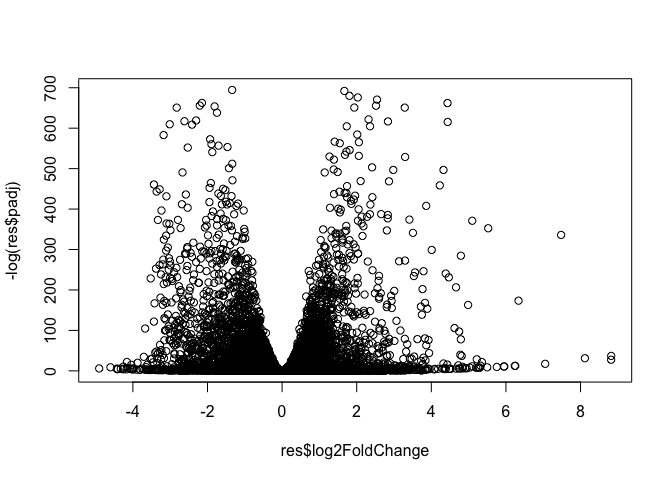
\includegraphics{Class06_Homework_files/figure-latex/unnamed-chunk-8-1.pdf}

Try it on ``1AKE''

\begin{Shaded}
\begin{Highlighting}[]
\KeywordTok{plot_B_factors}\NormalTok{(}\StringTok{"1AKE"}\NormalTok{, }\StringTok{"A"}\NormalTok{, }\StringTok{"CA"}\NormalTok{)}
\end{Highlighting}
\end{Shaded}

\begin{verbatim}
##   Note: Accessing on-line PDB file
##    PDB has ALT records, taking A only, rm.alt=TRUE
\end{verbatim}

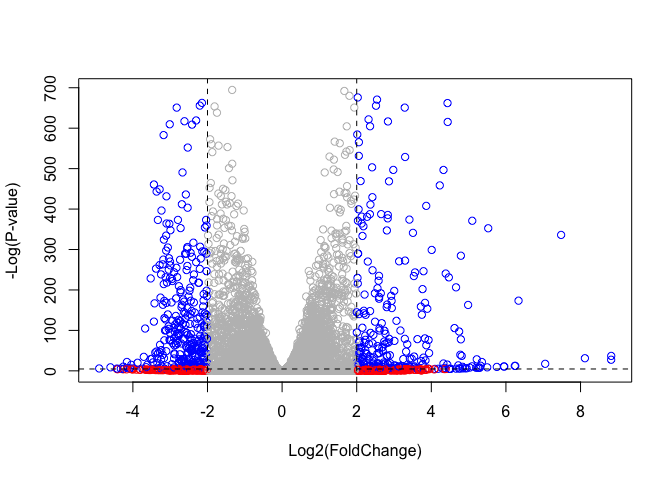
\includegraphics{Class06_Homework_files/figure-latex/unnamed-chunk-9-1.pdf}

Try it on ``1E4Y''

\begin{Shaded}
\begin{Highlighting}[]
\KeywordTok{plot_B_factors}\NormalTok{(}\StringTok{"1E4Y"}\NormalTok{, }\StringTok{"A"}\NormalTok{, }\StringTok{"CA"}\NormalTok{)}
\end{Highlighting}
\end{Shaded}

\begin{verbatim}
##   Note: Accessing on-line PDB file
\end{verbatim}

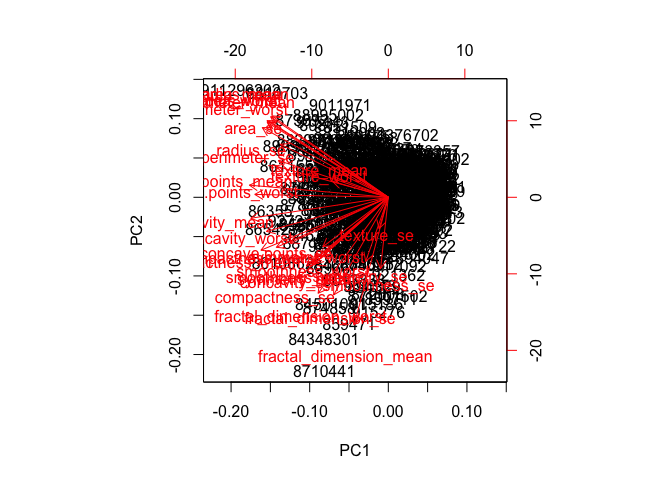
\includegraphics{Class06_Homework_files/figure-latex/unnamed-chunk-10-1.pdf}

Just for fun, a new PDB file: ``4RA4'' the Human Protein Kinase C Alpha

\begin{Shaded}
\begin{Highlighting}[]
\KeywordTok{plot_B_factors}\NormalTok{(}\StringTok{"1E4Y"}\NormalTok{, }\StringTok{"A"}\NormalTok{, }\StringTok{"CA"}\NormalTok{)}
\end{Highlighting}
\end{Shaded}

\begin{verbatim}
##   Note: Accessing on-line PDB file
\end{verbatim}

\begin{verbatim}
## Warning in get.pdb(file, path = tempdir(), verbose = FALSE): /var/folders/
## _6/v8hx8cc57x36zzxk__k_v96h0000gn/T//RtmpCgbv0x/1E4Y.pdb exists. Skipping
## download
\end{verbatim}

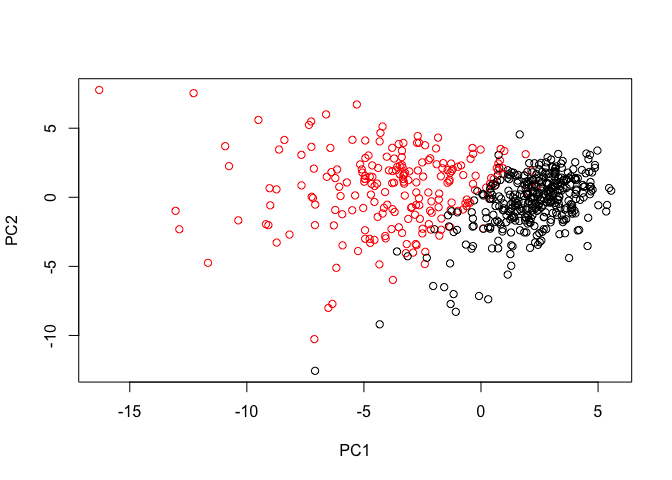
\includegraphics{Class06_Homework_files/figure-latex/unnamed-chunk-11-1.pdf}

What if I instead try to make a plot for chain B of ``4AKE''

\begin{Shaded}
\begin{Highlighting}[]
\KeywordTok{plot_B_factors}\NormalTok{(}\StringTok{"4AKE"}\NormalTok{, }\StringTok{"B"}\NormalTok{, }\StringTok{"CA"}\NormalTok{)}
\end{Highlighting}
\end{Shaded}

\begin{verbatim}
##   Note: Accessing on-line PDB file
\end{verbatim}

\begin{verbatim}
## Warning in get.pdb(file, path = tempdir(), verbose = FALSE): /var/folders/
## _6/v8hx8cc57x36zzxk__k_v96h0000gn/T//RtmpCgbv0x/4AKE.pdb exists. Skipping
## download
\end{verbatim}

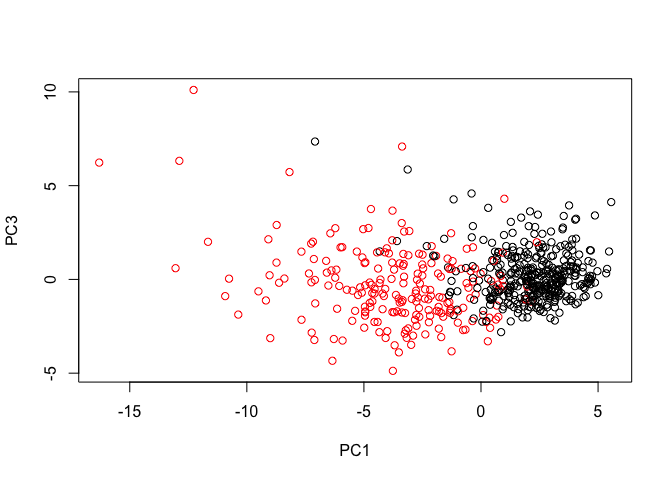
\includegraphics{Class06_Homework_files/figure-latex/unnamed-chunk-12-1.pdf}

It works :)


\end{document}
